\documentclass[a4paper,12pt]{article}
\usepackage[UTF8]{ctex}
\usepackage{listings}
\lstset{
	breaklines,                                 % 自动将长的代码行换行排版
	extendedchars=false,                        % 解决代码跨页时,章节标题,页眉等汉字不显示的问题
	backgroundcolor=\color[rgb]{0.96,0.96,0.96},% 背景颜色
	keywordstyle=\color{blue}\bfseries,         % 关键字颜色
	identifierstyle=\color{black},              % 普通标识符颜色
	commentstyle=\color[rgb]{0,0.6,0},          % 注释颜色
	stringstyle=\color[rgb]{0.58,0,0.82},       % 字符串颜色
	showstringspaces=false,                     % 不显示字符串内的空格
	numbers=left,                               % 显示行号
	captionpos=t,                               % title在上方(在bottom即为b)
	frame=single,                               % 设置代码框形式
	rulecolor=\color[rgb]{0.8,0.8,0.8},         % 设置代码框颜色
}  



%\usepackage{xeCJK}
\usepackage{times}
\usepackage{setspace}
\usepackage{fancyhdr}
\usepackage{graphicx}
\usepackage{wrapfig}
\usepackage{array}  
\usepackage{fontspec,xunicode,xltxtra}
\usepackage{titlesec}
\usepackage{titletoc}
\usepackage[titletoc]{appendix}
\usepackage[top=30mm,bottom=30mm,left=20mm,right=20mm]{geometry}
\usepackage{cite}
\usepackage{listings}
\usepackage[hidelinks]{hyperref}
\usepackage[framed,numbered,autolinebreaks,useliterate]{mcode} % 插入代码
\XeTeXlinebreaklocale "zh"
\XeTeXlinebreakskip = 0pt plus 1pt minus 0.1pt



%---------------------------------------------------------------------
%	章节标题设置
%---------------------------------------------------------------------
% \titleformat{\chapter}{\centering\zihao{-1}\heiti}{实验\chinese{chapter}}{1em}{}
% \titlespacing{\chapter}{0pt}{*0}{*6}

%---------------------------------------------------------------------
%	摘要标题设置
%---------------------------------------------------------------------
% \renewcommand{\abstractname}{\zihao{-3} 摘\quad 要}

%---------------------------------------------------------------------
%	参考文献设置
%---------------------------------------------------------------------
%\renewcommand{\bibname}{\zihao{2}{\hspace{\fill}参\hspace{0.5em}考\hspace{0.5em}文\hspace{0.5em}献\hspace{\fill}}}

%---------------------------------------------------------------------
%	引用文献设置为上标
%---------------------------------------------------------------------
\makeatletter
\def\@cite#1#2{\textsuperscript{[{#1\if@tempswa , #2\fi}]}}
\makeatother

%---------------------------------------------------------------------
%	目录页设置
%---------------------------------------------------------------------
%\titlecontents{chapter}[0em]{\songti\zihao{-4}}{\thecontentslabel\ }{}
%{\hspace{.5em}\titlerule*[4pt]{$\cdot$}\contentspage}
%\titlecontents{section}[2em]{\vspace{0.1\baselineskip}\songti\zihao{-4}}{\thecontentslabel\ }{}{\hspace{.5em}\titlerule*[4pt]{$\cdot$}\contentspage}
%\titlecontents{subsection}[4em]{\vspace{0.1\baselineskip}\songti\zihao{-4}}{\thecontentslabel\ }{}{\hspace{.5em}\titlerule*[4pt]{$\cdot$}\contentspage}


\usepackage{ctex}
\usepackage{listings}
\usepackage{xcolor}
\usas pd
import matplotlib.pyplot as plt
df=pd.read_excel("3-15.epackage{graphicx}
\usepackage{subfig}
\usepackage{array}
\usepackage{amsmath}
\usepackage{amssymb}
\begin{document}
\section{第一问}
源代码:
\begin{lstlisting}[language=python,breaklines]
	import numpy as np
	import pandas as pd
	import matplotlib.pyplot as plt
	df=pd.read_excel("3-15.xlsx")
	X=df.iloc[:,1]
	y=df.iloc[:,2]
	import statsmodels.api as sm
	X=sm.add_constant(X)
	ols=sm.OLS(y,X)
	models=ols.fit()
	models.params
\end{lstlisting}
out: 
\begin{figure}[htbp]
	\centering
	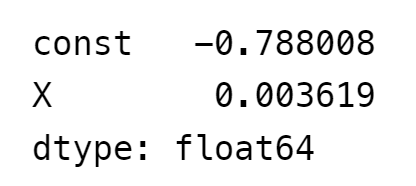
\includegraphics[scale=0.4]{out1.png}
	\caption{最小二乘回归结果}
\end{figure}
统计分析:

导入数据后将每小时用电量y作为因变量,将每月总用电量X作为自变量。从上图可以
读取最小二乘回归估计的结果,则经验回归方程为:

$$y=0.0036x-0.7880$$

\section{第二问}

源代码:
\begin{lstlisting}[language=python,breaklines]
	y_predict=models.predict()
	outliers=models.get_influence()
	ri=outliers.resid_studentized_internal
	plt.plot(y_predict,ri,'b.')
	plt.axhline(y=2,color="r",linestyle="--")
	plt.axhline(y=-2,color="r",linestyle="--")
	plt.xlabel("$\hat{y_i}$")
	plt.ylabel("$\hat{r_i}$")
\end{lstlisting}
out: 
\begin{figure}[htbp]
	\centering
	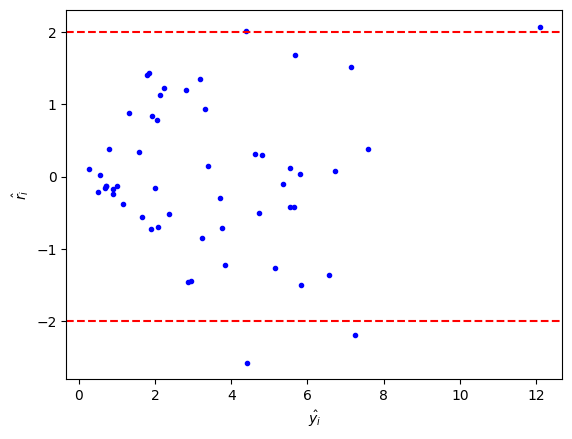
\includegraphics[scale=0.4]{out2.png}
	\caption{学生化残差图}
\end{figure}
统计分析:

学生化残差:$$r_i=\frac{\hat{e}}{\hat{\sigma}\sqrt{1-h_{ii}}}$$

其中,$\hat{e}=y-X\hat{\beta}$,$\hat{\sigma}=\frac{\hat{e}'\hat{e}}{n-1}$,$H=X(X'X)^{-1}X'\triangleq (h_{ij})$

从图中可以看出,几乎所有点都落在[-2,2]的区间内,所以Gauss-Markov假设对本例适用。

\section{第三问}

源代码:
\begin{lstlisting}
	import numpy as np
	X=df.iloc[:,1]
	y=df.iloc[:,2]
	u=np.sqrt(y)
	import statsmodels.api as sm
	X=sm.add_constant(X)
	ols1=sm.OLS(u,X)
	models1=ols1.fit()
	models1.params
\end{lstlisting}
out: 
\begin{figure}[htbp]
	\centering
	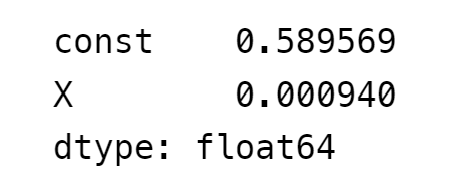
\includegraphics[scale=0.4]{out3.png}
	\caption{最小二乘回归结果}
\end{figure}
\begin{lstlisting}
	u_predict=models1.predict()
	outliers1=models1.get_influence()
	ri1=outliers1.resid_studentized_internal
	plt.plot(u_predict,ri1,'b.')
	plt.axhline(y=2,color="r",linestyle="--")
	plt.axhline(y=-2,color="r",linestyle="--")
	plt.xlabel("$\hat{y_i}$")
	plt.ylabel("$\hat{r_i}$")
\end{lstlisting}
out: 
\begin{figure}[htbp]
	\centering
	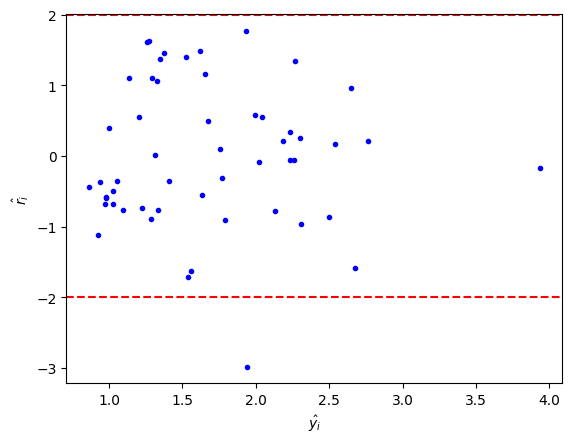
\includegraphics[scale=0.4]{out4.png}
	\caption{学生化残差图}
\end{figure}
统计分析:

由图可以读取最小二乘估计的结果,则经验回归方程为:

$$u=0.0009x+0.5896$$

学生化残差:$$r_i=\frac{\hat{e}}{\hat{\sigma}\sqrt{1-h_{ii}}}$$

其中,$\hat{e}=u-X\hat{\beta}$,$\hat{\sigma}=\frac{\hat{e}'\hat{e}}{n-1}$,$H=X(X'X)^{-1}X'\triangleq (h_{ij})$

从图中可以看出,几乎所有点都落在[-2,2]的区间内,所以Gauss-Markov假设对本例适用。

\section{第四问}

源代码:

\begin{lstlisting}[language=r,breaklines]
	library(xlsx)
	df<-read.xlsx("3-15.xlsx",1)
	X=as.matrix(df[,2])
	y=as.matrix(df[,3])
	library(MASS)
	bc<-boxcox(Y~X,data=df,lambda=seq(0,1,0.01))
	lambda<-bc$x[which.max(bc$y)]
	lambda
\end{lstlisting}

out: 0.53
\begin{figure}[htbp]
	\centering
	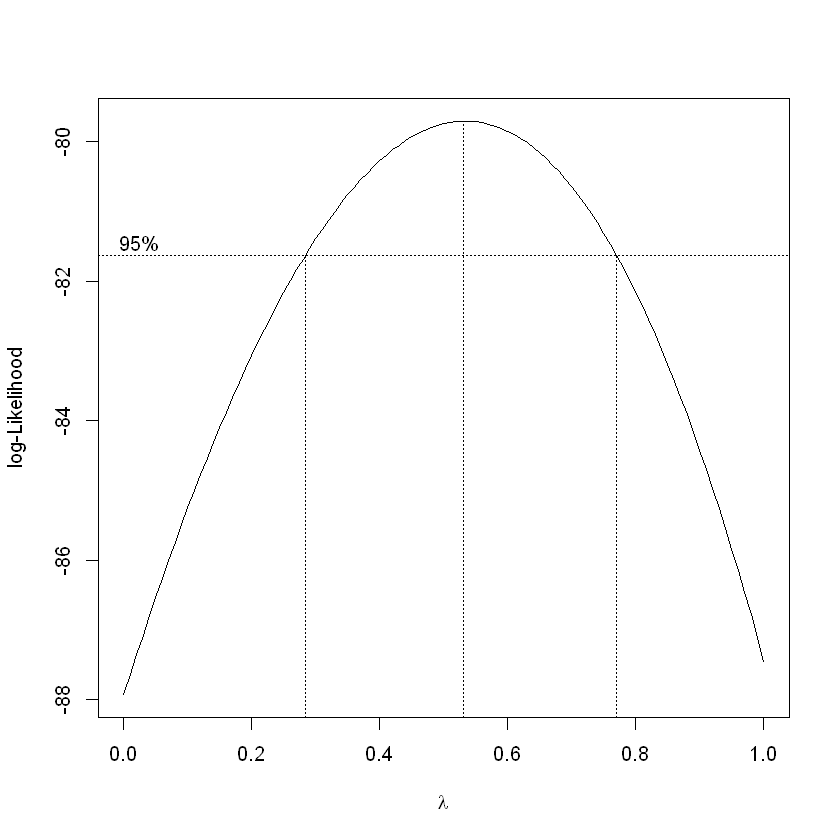
\includegraphics[scale=0.4]{out6.png}
	\caption{用似然法估计$\lambda$}
\end{figure}
统计分析:

从程序的输出结果可以看出,用似然法估计变换参数$\lambda$的结果为$\lambda=0.53$

Box-Cox变换:
\begin{equation*}
Y^{(\lambda)}=\left\{
	\begin{aligned}
		& \frac{Y^\lambda -1}{\lambda},lambda\neq 0\\
		& \ln{Y},lambda\neq 0
	\end{aligned}
\end{equation*}
\section{第五问}

源代码:
\begin{lstlisting}[language=python,breaklines]
	cook=outliers.cooks_distance
	plt.plot(cook[0],'b.')
	plt.axvline(x=7,color="g",linestyle="--")
	plt.axvline(x=25,color="g",linestyle="--")
	plt.axvline(x=49,color="g",linestyle="--")
	plt.axvline(x=51,color="g",linestyle="--")
\end{lstlisting}
out: 
\begin{figure}[htbp]
	\centering
	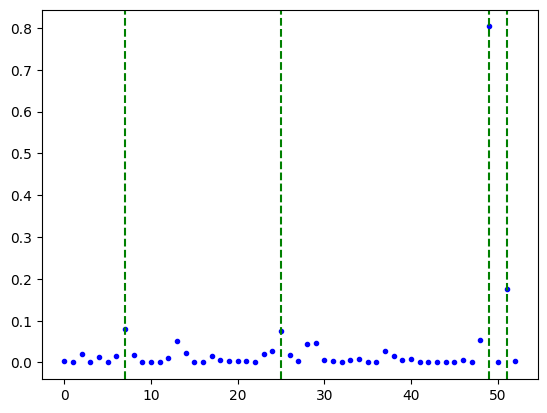
\includegraphics[scale=0.4]{out5.png}
	\caption{cook距离图}
\end{figure}
统计分析:

从图中可以看出,第8、26、50、52号点cook距离相对较大,尤其是第50、52号点。
可以认为第8、26、50、52号点对应的数据是强影响点。

cook距离求法:
$$D_i=\frac{1}{p}(\frac{h_{ii}}{1-h_{ii}})r_i^2$$
\end{document}